%% ----------------------------------------------------------------
%% InvestigationVision.tex
%% ---------------------------------------------------------------- 
\chapter{Investigation into Vision Algorithms} \label{Chapter:InvestigationVision}

\section{Comparison}
\inote{find some references to back these claims up}
\inote{Talk about how to compare images and TEST them all. Make a final comparison to decide on which will be used}
In computer vision, there are many different ways of comparing two similar images. These include the sum of absolute differences (S.A.D.) (\cite{Hamzah:DistanceDetection}), the sum of squared differences (S.S.D.), $\chi ^{2}$  and  normalised cross correlation (N.C.C.). Each of these methods will be explained and tested to compare them. All testing will use images seen in figure \ref{fig:StereoTest}. Each test uses the same size of image to compare to of 50$\times$ 50 pixels of the same part of the image. 

\begin{figure}
\centering
\subfigure[Left Image]{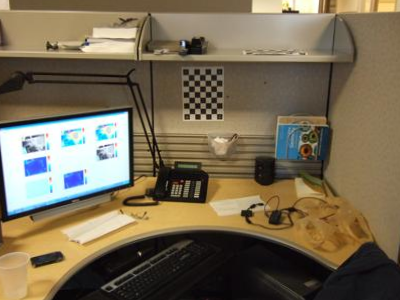
\includegraphics[scale=0.4]{./Figures/deskLeft.png} }
\subfigure[Right Image]{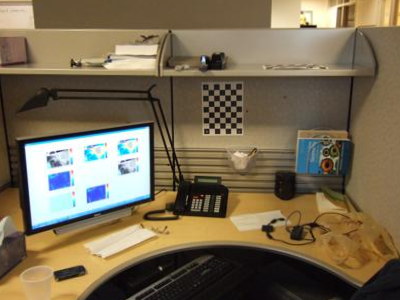
\includegraphics[scale=0.4]{./Figures/deskRight.png} }
\caption{Stereoscopic Test Images from MATLAB Examples}
\label{fig:StereoTest}
\end{figure}


%Explanation of how they work
\inote{Maybe do a basic 5x5 example for each?}
\subsection{Sum of Absolue Differences}

Given two indentically sized matricies, $A, B$ of dimensions $I,J$, SAD is defined as
\begin{equation} \label{eq:SAD}
SAD = \sum\limits_{i=0}^{I-1} \sum\limits_{j=0}^{J-1} A[i,j] - B[i,j] 
\end{equation}

This method takes each sub image and subtracts the observed sub image from the expected. All differences are then added together. This algorithm is simple and requires a small amount of computation. The algorithm returns values where a small result means the two images are well matched.

\subsection{Sum of Squared Differences}
\begin{equation}\label{eq:SSD}
SSD = \sum\limits_{i=0}^{I-1} \sum\limits_{j=0}^{J-1} (A[i,j] - B[i,j] )^2
\end{equation}

This is very similar to S.A.D. but adds more complexity by squaring each difference. This removes the ability of equally different but opposite differences cancelling each other out (grey to white of one pixel will cancel out a white to grey difference in the other). Again, a low result is a match in this case.

\inote{sort chi out}
\subsection{$\chi ^{2}$ }
$\chi ^{2}$ is ``Insert definition here". For use with images the equation can be adapted to \ref{eq:ChiSquare}. 

\begin{equation} \label{eq:ChiSquare}
\chi ^{2} = \sum\limits_{i=0}^{I-1} \sum\limits_{j=0}^{J-1}\frac{(A[i,j] - B[i,j])^2}{(A[i,j]+B[i,j])/2}
\end{equation}


\subsection{NCC}
\begin{equation}\label{eq:NCC}
NC(x,y) =  \sum\limits_i \sum\limits_j A[i+x, j+y]\times B[i,j] - I\times 
\end{equation}
NCC is very similar to cross correlation, but normalised to reduce the error if one image is brighter than the other. It is common in computer vision \cite{}


%test and compare
\subsection{Comparison}



\section{Range Finding}
\inote{Derive the range finding eauations and test the fuck out of it}

\subsection{Derivations}

By using two images sepearted by a horizontal difference, the range of an object can be found given some characteristics of the camera. The following is a derivation of the equations used to calculate distance. 

The problem is broken down into 3
\begin{enumerate}
\item Object is between the cameras (Figure \ref{problem_between})
\item Object is directly infront of a camera
\item Object is in left or right hand sides of both images
\end{enumerate}

\begin{figure}
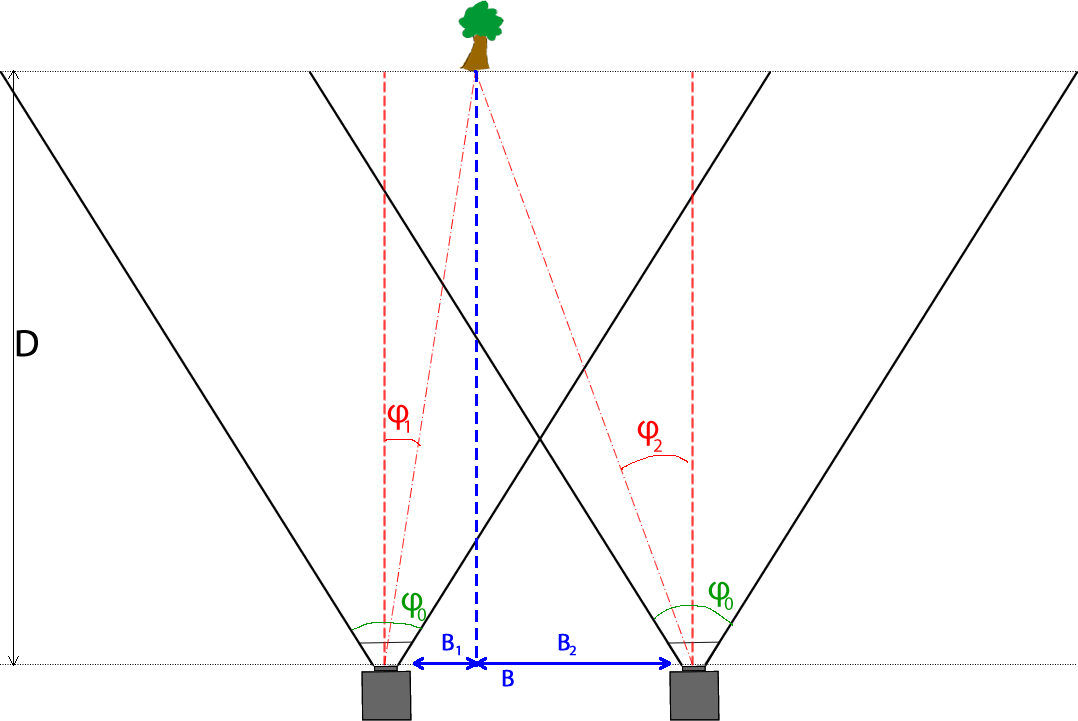
\includegraphics[width=\textwidth,height=\textheight,keepaspectratio]{Figures/problem1.png}
\caption{Problem 1 - Object is between the Cameras}
\label{problem_between}
\end{figure}

\subsubsection{Object is between the Cameras}
Derivation from \cite{Mrovlje:Distance_Stereoscopic}.
\begin{equation} \label{eq:B}
B = B_{1} + B_{2} = D\tan(\varphi_{1}) + D\tan(\varphi_{2})
\end{equation}

\begin{equation} \label{eq:D}
D = \frac{B}{\tan(\varphi_{1}) + \tan(\varphi_{2})}
\end{equation}


\begin{figure}
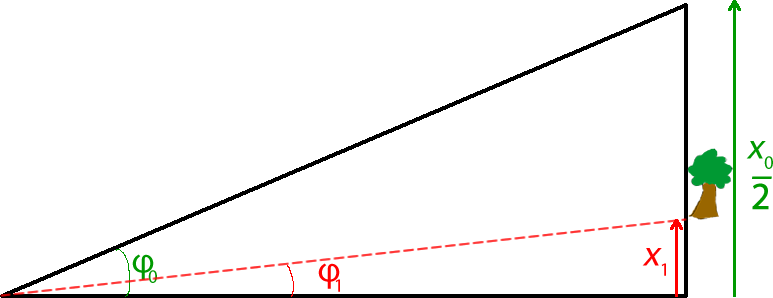
\includegraphics[width=\textwidth,height=\textheight,keepaspectratio]{Figures/left_simplified.png}
\caption{Problem 1 : Left Camera Simplified}
\label{Left_Simplified}
\end{figure}

\begin{equation} \label{eq:phi}
D\tan(\frac{\varphi_{0}}{2}) = x_{0} / 2
\end{equation}

\begin{equation} \label{eq:phi1}
D\tan(\varphi_1) = x_1
\end{equation}

Dividing \eqref{eq:phi1} by \eqref{eq:phi}

\begin{equation} \label{eq:tanovertan}
\frac{\tan(\varphi_1)}{\tan(\frac{\varphi_0}{2})} = \frac{2x_1}{x_0}
\end{equation}

\begin{equation} \label{eq:phionesolved}
\tan(\varphi_1) = \frac{2x_1\tan(\frac{\varphi_0}{2})}{x_0}
\end{equation}

It can also be shown that for the right camera:

\begin{equation} \label{eq:phitwosolved}
\tan(\varphi_2) = \frac{-2x_2\tan(\frac{\varphi_0}{2})}{x_0}
\end{equation}

Substitution equations \eqref{eq:phionesolved} and \eqref{eq:phitwosolved} into \eqref{eq:D} gives

\begin{equation} \label{eq:Distance1}
D = \frac{Bx_0}{2\tan(\frac{\varphi_0}{2})(x_1 - x_2)}
\end{equation}


\subsubsection{Object is infront of a camera}


\subsubsection{Object is to the same side in each camera}

\begin{figure}
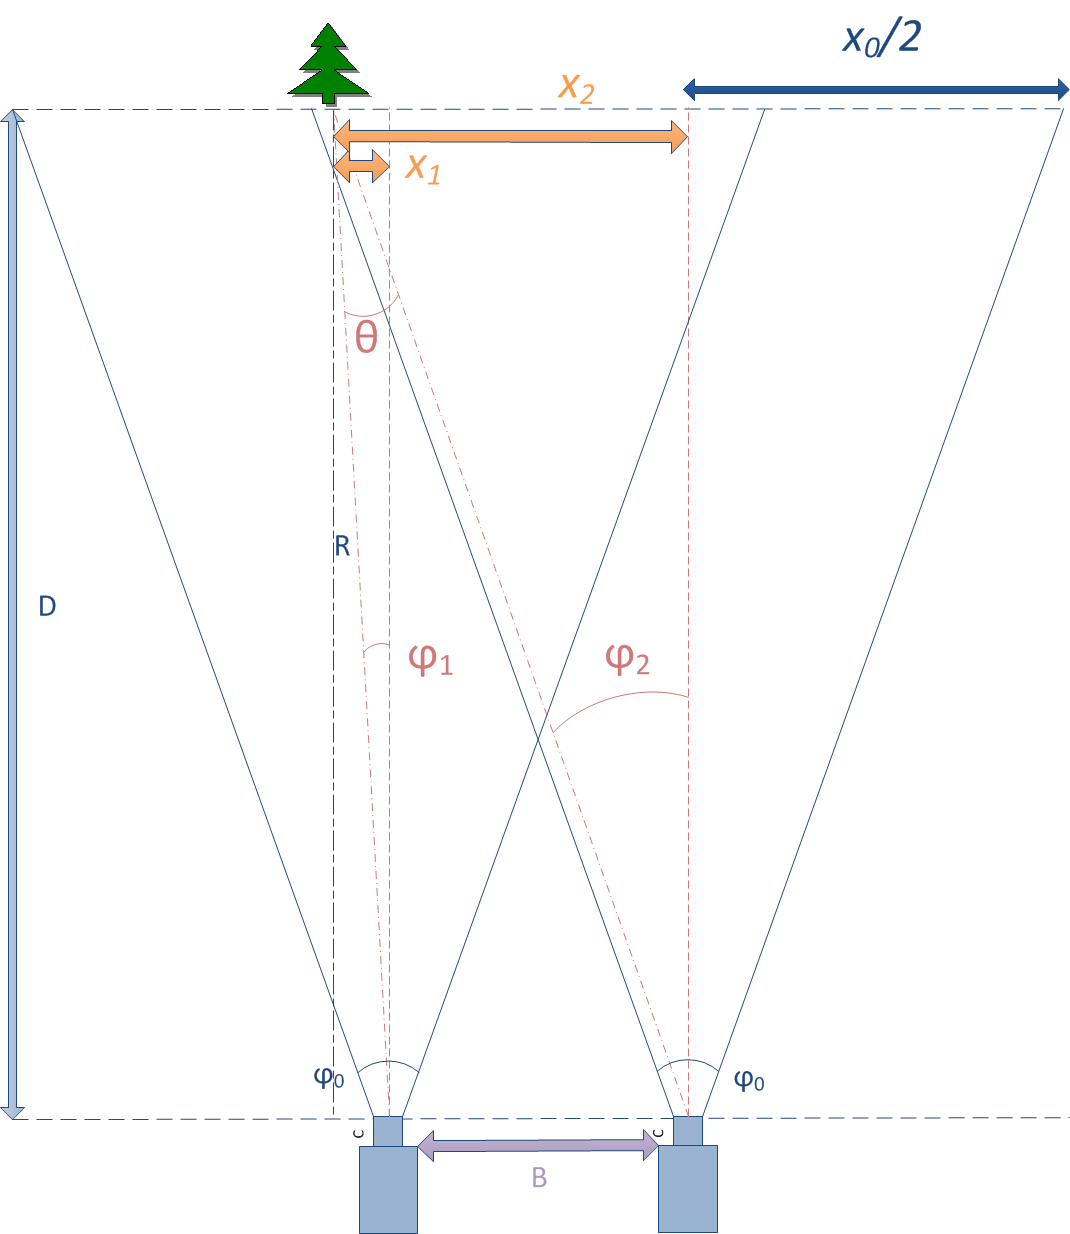
\includegraphics[width=\textwidth,height=\textheight,keepaspectratio]{Figures/problem2.png}
\caption{Problem 3 - Object is to the same side in both cameras}
\label{problem_toleft}
\end{figure}
